\documentclass[10pt]{beamer}
\usepackage[utf8]{inputenc}
\usepackage[T1]{fontenc}
\usepackage{lmodern}
\usepackage{amsmath,amssymb,amsthm}
\usepackage{booktabs}
\usepackage{xcolor}
\usepackage{tikz}
\usetikzlibrary{positioning,arrows.meta}
\usepackage{enumitem}

\usetheme{Madrid}
\usecolortheme{whale}

% Colors from original paper
\definecolor{lblue}{RGB}{55,138,221}
\definecolor{rred}{RGB}{226,75,74}
\definecolor{lgray}{RGB}{245,244,241}
\definecolor{mgray}{RGB}{90,90,90}

% Macros
\newcommand{\Lopt}[1]{{\color{lblue}\textbf{#1}}}
\newcommand{\Ropt}[1]{{\color{rred}\textbf{#1}}}
\newcommand{\Gv}[1]{\mathcal{G}(#1)}
\newcommand{\tmp}[1]{t\!\left(#1\right)}

% TikZ styles for game trees
\tikzset{
  nd/.style={circle, draw, fill=white, inner sep=2pt, minimum size=14pt, font=\scriptsize},
  lf/.style={circle, draw=mgray, fill=lgray, inner sep=1.5pt, minimum size=9pt},
  Le/.style={-{Stealth[length=4pt]}, lblue, semithick},
  Re/.style={-{Stealth[length=4pt]}, rred, semithick},
  lbl/.style={font=\tiny},
  gametree/.style={scale=0.92, transform shape}
}

\title{Directed Tree Ascent}
\subtitle{A Partizan Combinatorial Game on Edge-Labelled Rooted Binary Trees}
\author{IE619 --- Combinatorial Game Theory (2025)}
\date{}

\begin{document}

% ==================== Title Slide ====================
\begin{frame}
  \titlepage
\end{frame}

% ==================== Game Definition ====================
\begin{frame}{Game Definition}
  \begin{definition}[Directed Tree Ascent (DTA)]
    A finite rooted binary tree with each edge labelled \Lopt{L} or \Ropt{R}, directed from parent to child. 
    A token starts at the root.
    
    \smallskip
    \Lopt{Left} moves the token along any adjacent \Lopt{L}-edge to a child.
    
    \smallskip
    \Ropt{Right} moves along any adjacent \Ropt{R}-edge to a child.
    
    \smallskip
    Normal play: the player unable to move loses.
  \end{definition}
  
  Multiple independent trees are combined using the \textbf{disjunctive sum}.
\end{frame}

% ==================== Design Criteria ====================
\begin{frame}{Nine Design Criteria}
  \begin{center}
    \begin{tabular}{@{}p{3.4cm}l@{}}
      \toprule
      Criterion & DTA \\
      \midrule
      No target condition   & last-to-move wins \checkmark \\
      Novel                 & no prior literature \checkmark \\
      Named                 & ``Directed Tree Ascent'' \checkmark \\
      Scalable              & arbitrary depth / branching \checkmark \\
      Disjunctive sum       & independent trees sum freely \checkmark \\
      One-liner per player  & yes \checkmark \\
      Partizan              & distinct \Lopt{L}/\Ropt{R} edges \checkmark \\
      Board feel            & path vs.\ branch strategy tension \checkmark \\
      Interesting math      & $\mathbb{Z}$, switches, $*$, $\uparrow$ \checkmark \\
      \bottomrule
    \end{tabular}
  \end{center}
\end{frame}

% ==================== Recursive Value ====================
\begin{frame}{Recursive Value Formula}
  For a node $v$ with \Lopt{L}-children $\mathcal{L}(v)$ and \Ropt{R}-children $\mathcal{R}(v)$:
  \[
    \Gv{v} = \bigl\{ \Gv{c} : c \in \mathcal{L}(v) \;\big|\; 
                     \Gv{c} : c \in \mathcal{R}(v) \bigr\}
  \]
  Base case: leaf $\Gv{\ell} = \{ | \} = 0$.
\end{frame}

% ==================== Basic Positions ====================
\begin{frame}{Basic Positions}
  \begin{columns}[T]
    \column{0.5\textwidth}
      \centering
      \textbf{\Lopt{L}-path} $\to 1$
      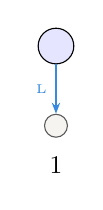
\begin{tikzpicture}[gametree]
        \node[nd,fill=blue!10] (r) at (0,0) {};
        \node[lf] (l) at (0,-1.1) {};
        \draw[Le] (r)--(l) node[midway,left,lbl]{L};
        \node[below=4pt of l] {$1$};
      \end{tikzpicture}

      \vspace{12pt}
      \textbf{Star} $*= \{0|0\}$
      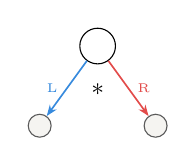
\begin{tikzpicture}[gametree]
        \node[nd] (r) at (0,0) {};
        \node[lf] (l1) at (-0.8,-1.1) {};
        \node[lf] (l2) at (0.8,-1.1) {};
        \draw[Le] (r)--(l1) node[midway,left,lbl]{L};
        \draw[Re] (r)--(l2) node[midway,right,lbl]{R};
        \node[below=4pt of r] {$*$};
      \end{tikzpicture}

    \column{0.5\textwidth}
      \centering
      \textbf{Up} $\uparrow = \{0|*\}$
      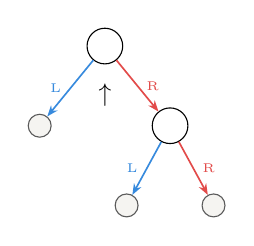
\begin{tikzpicture}[gametree]
        \node[nd] (r) at (0,0) {};
        \node[lf] (l) at (-0.9,-1.1) {};
        \node[nd] (m) at (0.9,-1.1) {};
        \node[lf] (ll) at (0.3,-2.2) {};
        \node[lf] (rr) at (1.5,-2.2) {};
        \draw[Le] (r)--(l) node[midway,left,lbl]{L};
        \draw[Re] (r)--(m) node[midway,right,lbl]{R};
        \draw[Le] (m)--(ll) node[midway,left,lbl]{L};
        \draw[Re] (m)--(rr) node[midway,right,lbl]{R};
        \node[below=4pt of r] {$\uparrow$};
      \end{tikzpicture}

      \vspace{12pt}
      \textbf{Switch} $\pm 1$
      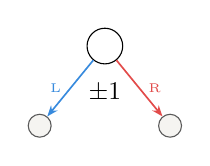
\begin{tikzpicture}[gametree]
        \node[nd] (r) at (0,0) {};
        \node[lf] (l) at (-0.9,-1.1) {};
        \node[lf] (rr) at (0.9,-1.1) {};
        \draw[Le] (r)--(l) node[midway,left,lbl]{L};
        \draw[Re] (r)--(rr) node[midway,right,lbl]{R};
        \node[below=4pt of r] {$\pm 1$};
      \end{tikzpicture}
  \end{columns}
\end{frame}

% ==================== Value Catalogue ====================
\begin{frame}{Value Catalogue}
  \small
  \begin{tabular}{@{}p{2.9cm}llc@{}}
    \toprule
    Tree shape & $\Gv{\cdot}$ & Type & $\tmp{\cdot}$ \\
    \midrule
    $\Lopt{L}^n$ path          & $n$          & integer       & $-\infty$ \\
    $\Ropt{R}^n$ path          & $-n$         & integer       & $-\infty$ \\
    $n$ L-leaves + $n$ R-leaves & $\pm n$     & switch        & $n$ \\
    L-leaf + R-leaf            & $*$          & fuzzy         & $0$ \\
    L-leaf + R$\to\{$L,R$\}$   & $\uparrow$   & infinitesimal & $0$ \\
    Alternating (odd)          & $1$          & integer       & $-\infty$ \\
    \bottomrule
  \end{tabular}
\end{frame}

% ==================== Structural Theorems ====================
\begin{frame}{Structural Theorems}
  \begin{theorem}[Monochromatic paths are integers]
    $\Gv{P^n_L} = n$ and $\Gv{P^n_R} = -n$.
  \end{theorem}

  \begin{theorem}[Symmetric branch gives switch]
    Root with $n$ \Lopt{L}-leaves and $n$ \Ropt{R}-leaves: $\Gv{T_{\pm n}} = \pm n$.
  \end{theorem}
\end{frame}

\begin{frame}{Infinitesimals}
  \begin{definition}
    $T_* = \{0 \mid 0\} = *$
    
    $T_\uparrow = \{0 \mid *\} = \uparrow$
  \end{definition}

  \begin{theorem}
    $\uparrow \parallel *$ (they are incomparable).
  \end{theorem}

  \textbf{Important consequence:} Temperature-based strategies can fail when both $*$ and $\uparrow$ appear in a sum.
\end{frame}

% ==================== Outcome Classes ====================
\begin{frame}{Outcome Classes}
  \[
    \Gv{T}\ 
    \begin{cases}
      > 0  & \Rightarrow \mathcal{L} \quad \text{(Left wins regardless)}\\
      < 0  & \Rightarrow \mathcal{R} \quad \text{(Right wins regardless)}\\
      = 0  & \Rightarrow \mathcal{P} \quad \text{(second player wins)}\\
      \| 0 & \Rightarrow \mathcal{N} \quad \text{(first player wins)}
    \end{cases}
  \]

  \vspace{10pt}
  \small
  \begin{tabular}{@{}llll@{}}
    \toprule
    Position & Value & Outcome & Winner \\
    \midrule
    $P^3_L$         & $3$      & $\mathcal{L}$ & Left always \\
    $T_{\pm 2}$     & $\pm 2$  & $\mathcal{N}$ & First player \\
    $T_*$           & $*$      & $\mathcal{N}$ & First player \\
    $T_\uparrow$    & $\uparrow$ & $\mathcal{L}$ & Left always \\
    $P^2_L + P^2_R$ & $0$      & $\mathcal{P}$ & Second player \\
    \bottomrule
  \end{tabular}
\end{frame}

% ==================== Open Problems ====================
\begin{frame}{Open Problems}
  \begin{enumerate}[label=\small(\roman*)]
    \item Full closed-form value characterisation for arbitrary trees
    \item Computational complexity of outcome in disjunctive sums
    \item Misère version of DTA
    \item $k$-ary generalisation with $k$ colours
    \item Behaviour on infinite trees
  \end{enumerate}
  
  \bigskip
  \small References: \emph{Winning Ways}, \emph{On Numbers and Games}, Siegel's \emph{Combinatorial Game Theory}.
\end{frame}

\begin{frame}
  \centering
  \Huge Thank You!
  
  \bigskip
  \Large Questions?
  
  \bigskip\bigskip
  \Lopt{Left} and \Ropt{Right} are ready to ascend the tree!
\end{frame}

\end{document}